In this section the experimental results are presented. We evaluate the performance on six sets of games:
\begin{itemize}
	\item the minepump games,
	\item the elevator games,
	\item random games of type 1 with an increasing $\lambda$,
	\item random games of type 2 with an increasing $\lambda$,
	\item random games of type 3 with an increasing $\lambda$ and
	\item random games of type 1 with an increasing number of configuration.
\end{itemize}

We present the times it took to solve a VPG. For an independent approach this means the sum of the times it taken to solve every projection of the VPG. For a collective approach this means simply means the solve time for the VPG. In either case we only measure the solve time; parsing, projecting and solution printing is excluded from the evaluation.

The exact times can be found in appendix \ref{appendix:resultsexact}, in this section the results are visualized and presented in a way such that we can easily compare independent and collective approaches. We have four independent approaches:
\begin{itemize}
	\item Recursive algorithm (global),
	\item Recursive algorithm (local),
	\item fixed-point iteration (global) and
	\item fixed-point iteration (local).
\end{itemize}
For every set of problems we present four charts; for every independent approaches we present a chart where its performance is compared to one or two collective algorithms. We compare the performance of the recursive algorithm for VPGs with the performance of the original recursive algorithm and the performance of the incremental pre-solve algorithm with the performance of the fixed-point iteration algorithm. In every chart the solve times are divided by the independent solve times to visualize how much better or worse the collective variants perform.

The following legend holds for all charts presented in this section:
\begin{itemize}[\ ]
	\item Independent approaches:
	\begin{itemize}[\ ]
\item \raisebox{.7\height}{
\begin{tikzpicture}
\path[line width=2pt,color=cyan] (19,20) edge (20,20);
\end{tikzpicture}} Recursive algorithm for parity games (global)
\item \raisebox{.7\height}{
\begin{tikzpicture}
\path[line width=2pt,color=violet] (19,20) edge (20,20);
\end{tikzpicture}} Fixed-point iteration algorithm for parity games (global)
\item \raisebox{.7\height}{
\begin{tikzpicture}
	\path[dashed,line width=2pt,color=cyan] (19,20) edge (20,20);
	\end{tikzpicture}} Recursive algorithm for parity games (local)
\item \raisebox{.7\height}{
\begin{tikzpicture}
	\path[dashed,line width=2pt,color=violet] (19,20) edge (20,20);
	\end{tikzpicture}} Fixed-point iteration algorithm for parity games (local)
\end{itemize}
\item Collective approaches:
\begin{itemize}[\ ]
\item \raisebox{.7\height}{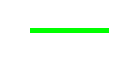
\begin{tikzpicture}
\path[line width=2pt,color=green] (19,20) edge (20,20);
\end{tikzpicture}} Recursive algorithm for VPGs with a symbolic representation of configurations (global)
\item \raisebox{.7\height}{
\begin{tikzpicture}
\path[line width=2pt,color=red] (19,20) edge (20,20);
\end{tikzpicture}} Recursive algorithm for VPGs with an explicit representation of configurations (global)
\item \raisebox{.7\height}{
\begin{tikzpicture}
\path[line width=2pt,color=orange] (19,20) edge (20,20);
\end{tikzpicture}} Incremental pre-solve algorithm (global)
\item \raisebox{.7\height}{
\begin{tikzpicture}
\path[dashed,line width=2pt,color=green] (19,20) edge (20,20);
\end{tikzpicture}} Recursive algorithm for VPGs with a symbolic representation of configurations (local)
\item \raisebox{.7\height}{
\begin{tikzpicture}
\path[dashed,line width=2pt,color=red] (19,20) edge (20,20);
\end{tikzpicture}} Recursive algorithm for VPGs with an explicit representation of configurations (local)
\item \raisebox{.7\height}{
\begin{tikzpicture}
\path[dashed,line width=2pt,color=orange] (19,20) edge (20,20);
\end{tikzpicture}} Incremental pre-solve algorithm (local)
\end{itemize}
\end{itemize}
All the experiments are ran on a Linux x64 operating system with an Intel i5-4570 @ 3.20 GHz processor and 8GB of DDR3 RAM.
\subsection{Model checking examples}
Figures \ref{fig:results_minepump} and \ref{fig:results_elevator} show the solving times of the algorithms when applied to the model checking examples.
\begin{figure}[H]
	\centering
	\begin{multicols}{2}
		\input{"results/minepump/Zlnk product based_Zlnk fam based - explicit_Zlnk fam based - symbolic_"}\\\vfill
		\input{"results/minepump/Zlnk local product based_Zlnk fam based - explicit local_Zlnk fam based - symbolic local_"}\\
		\input{"results/minepump/Fixed-point product based_Incremental pre-solve_"}\\\vfill
		\input{"results/minepump/Fixed-point local product based_Incremental pre-solve local_"}
	\end{multicols}
	\caption{Running times on the minepump games, times are normalized}
	\label{fig:results_minepump}
\end{figure}%
For the minepump example we see that the recursive algorithm for VPGs using a symbolic representation of configurations performs particularly well. For the elevator example we find a similar result, however for these games we also find a good performance for the incremental pre-solve algorithm. There is no clear difference between the relative performances of the global algorithms and the local algorithms.
\begin{figure}[H]
	\centering
	\begin{multicols}{2}
		\input{"results/elevator/Zlnk product based_Zlnk fam based - explicit_Zlnk fam based - symbolic_"}\\\vfill
		\input{"results/elevator/Zlnk local product based_Zlnk fam based - explicit local_Zlnk fam based - symbolic local_"}\\
		\input{"results/elevator/Fixed-point product based_Incremental pre-solve_"}\\\vfill
		\input{"results/elevator/Fixed-point local product based_Incremental pre-solve local_"}
	\end{multicols}
	\caption{Running times on the elevator games, times are normalized}
	\label{fig:results_elevator}
\end{figure}%

\subsection{Random games}
Figure \ref{fig:results_type1} shows the performance of the algorithms on type 1 games. The recursive algorithms for VPGs performh quite well, even though there are a few instances where the performance is worse that the independent approach. The symbolic variant performs quite a bit better than the explicit variant. The relative performance of the local variants of the recursive algorithms is about the same as the relative performance of the global variants. 

For the incremental pre-solve algorithm we do see a big difference between a local and global approach. The global variant performs well only for games 90 and up. The local variant, however, performs well for nearly all the games. Furthermore, even for the games where the global variant performs well does the local variant perform even better.
\begin{figure}[H]
	\centering
	\begin{multicols}{2}
		\input{"results/FF_randomgames/Zlnk product based_Zlnk fam based - explicit_Zlnk fam based - symbolic_"}\\
		\input{"results/FF_randomgames/Zlnk local product based_Zlnk fam based - explicit local_Zlnk fam based - symbolic local_"}\\
		\input{"results/FF_randomgames/Fixed-point product based_Incremental pre-solve_"}\\
		\input{"results/FF_randomgames/Fixed-point local product based_Incremental pre-solve local_"}
	\end{multicols}
	\caption{Running times on random games of type 1 with $\lambda = \frac{\textit{game nr}}{100}$, times are normalized}
	\label{fig:results_type1}
\end{figure}%


Figure \ref{fig:results_type2} shows the performance of the algorithms on type 1 games. For the recursive algorithms we see that the explicit variant takes over from the symbolic variant. This is to be expected since these games have edge guards that are not created from features but created by picking random configurations. Both variants still perform somewhat better than the independent approach. Again we do not find a significant difference between the global and local approach.

For the incremental pre-solve algorithm we find a similar result as with type 1 games. The global variant performs well only when $\lambda$ is high. The local variant performs significantly better and performs well for almost all games.
\begin{figure}[H]
	\centering
	\begin{multicols}{2}
		\input{"results/FC_randomgames/Zlnk product based_Zlnk fam based - explicit_Zlnk fam based - symbolic_"}\\
		\input{"results/FC_randomgames/Zlnk local product based_Zlnk fam based - explicit local_Zlnk fam based - symbolic local_"}\\
		\input{"results/FC_randomgames/Fixed-point product based_Incremental pre-solve_"}\\
		\input{"results/FC_randomgames/Fixed-point local product based_Incremental pre-solve local_"}
	\end{multicols}
	\caption{Running times on random games of type 2 with $\lambda = \frac{\textit{game nr}}{100}$, times are normalized}
	\label{fig:results_type2}
\end{figure}%

Figure \ref{fig:results_type3} shows the performance of the algorithms on type 3 games. For these games we see the symbolic variant of the recursive algorithm performing worse that the independent approach for almost all games. The explicit variant still performs significantly better that the symbolic variant and performs somewhat better than the independent approach. Again we do not find a significant difference between the global and local approach.

The global incremental pre-solve algorithm performs worse than the independent approach for almost all games. Notably for these games we do not find a significant increase in relative performance when using a local variant.

Notably, the explicit recursive algorithm seems to be the only algorithm unaffected by the fact that the guard sets of type 3 games vary wildly (they are distributed using a beta distribution). Maybe surprisingly, the incremental pre-solve algorithm is affected heavily by this. This is most likely because there are a lot fewer edges that admit all configurations and therefore player $\alpha$ will probably win less vertices in a pessimistic game for player $\alpha$.

\begin{figure}[H]
	\centering
	\begin{multicols}{2}
		\input{"results/BC_randomgames/Zlnk product based_Zlnk fam based - explicit_Zlnk fam based - symbolic_"}\\\vfill
		\input{"results/BC_randomgames/Zlnk local product based_Zlnk fam based - explicit local_Zlnk fam based - symbolic local_"}\\
		\input{"results/BC_randomgames/Fixed-point product based_Incremental pre-solve_"}\\\vfill
		\input{"results/BC_randomgames/Fixed-point local product based_Incremental pre-solve local_"}
	\end{multicols}
	\caption{Running times on random games of type 3 with $\lambda = \frac{\textit{game nr}}{100}$, times are normalized}
	\label{fig:results_type3}
\end{figure}%

\subsection{Scaling}
Figure \ref{fig:results_scalegames} shows the performance of the algorithms on type 1 games where the number of configurations increase exponentially in the x-axis of the charts. For the recursive algorithm we see that the collective approach starts outperforming the independent approach around $2^4$ configurations. As the number of configurations grow we see that the symbolic variant keeps increasing in relative performance while the explicit variants relative performance starts to flatten. This is to be expected because the performance of the explicit variant always scales linearly in the number of configurations. In the worst case the symbolic variant scales quadratically in the number of configurations, however when the sets of configurations can be represented efficiently it scales much better and in this case sublinear (since the performance of the local variant keeps increasing relative to the explicit variant).

The global incremental pre-solve algorithms does not increase notably in relative performance when the number of configurations increases. However, the relative performance of the local variant does increase in performance when the number of configurations increases. The recursion of the incremental pre-solve algorithm can be conceptualized as a tree where at every node the algorithm tries to increase the pre-solved vertices. The local variant can terminate when at some node the vertex that is being locally solved is found. In such a case the whole subtree of that node is longer computed. When the number of configurations grow then potentially the size of this subtree also grows. The fact that the local incremental pre-solve algorithm scales well in the number of configurations is most likely because the algorithm can terminate early for a relatively large set of configurations.

\begin{figure}[H]
	\centering
	\begin{multicols}{2}
		\input{"results/randomscalegames/Zlnk product based_Zlnk fam based - explicit_Zlnk fam based - symbolic_"}\\\vfill
		\input{"results/randomscalegames/Zlnk local product based_Zlnk fam based - explicit local_Zlnk fam based - symbolic local_"}\\
		\input{"results/randomscalegames/Fixed-point product based_Incremental pre-solve_"}\\\vfill
		\input{"results/randomscalegames/Fixed-point local product based_Incremental pre-solve local_"}
	\end{multicols}
	\caption{Running times on random games of type 1 with $\lambda = 0.92$ and the number of features equal to the $\textit{game nr}$, times are normalized}
	\label{fig:results_scalegames}
\end{figure}%

\subsection{Comparison}
From the experimental results we observe that the symbolic variant of the recursive algorithms for VPGs performs well for the model verification problems. For type 1 random games it also performs well and particularly scales very well in the number of configurations. For type 2 and 3 games the sets of configurations can no longer be efficiently represented symbolically. Earlier we hypothesised that the recursive algorithm for VPGs could perform well if we can attract many configurations simultaneously. For every VPG we measure the average number of configurations that were attracted simultaneously. We measure this relative to the total number of configurations in the VPG. This gives a number for every VPG. For every set of VPGs we average this number to get an average set size for every problem set. These values indicate how many configuration were attracted simultaneously, they are presented in Table \ref{tab_attracted_set_size}. We see that this number somewhat predicts the performance of the recursive algorithms.

\begin{table}[h]
	\centering
	\begin{tabular}{|l|l|l|l|l|}
		\hline
		Minepump& 46\%\\ \hline
		Elevator& 51\%\\ \hline
		Type 1, scaling in $\lambda$& 61\%\\ \hline
		Type 2, scaling in $\lambda$& 55\%\\ \hline
		Type 3, scaling in $\lambda$& 22\%\\ \hline
		Type 1, scaling in \# confs& 72\%\\ \hline
	\end{tabular}
	\caption{Relative size of attracted sets}
	\label{tab_attracted_set_size}
\end{table}

After comparing independent and collective approaches we compare the performances of the algorithms overall.

First we compare the independent algorithms. Table \ref{tab_compare_independent_algs} shows for every set of VPGs how long on average it took each algorithm to solve a VPG in that set.
\begin{table}[h]
	\centering
	\begin{tabular}{|l|l|l|l|l|}
		\hline
		& Recursive &Recursive & Fixed-point & Fixed-point\\
		& global & local & global & local \\
		\hline
		Minepump& 113 ms& 97 ms& 1852 ms& 1775 ms\\ \hline
		Elevator& 11374 ms& 9420 ms& 1061198 ms& 301363 ms\\ \hline
		Type 1, scaling in $\lambda$& 75 ms& 69 ms& 2147 ms& 2056 ms\\ \hline
		Type 2, scaling in $\lambda$& 75 ms& 71 ms& 2986 ms& 2900 ms\\ \hline
		Type 3, scaling in $\lambda$& 74 ms& 77 ms& 2496 ms& 2048 ms\\ \hline
		Type 1, scaling in \# confs& 590 ms& 529 ms& 7857 ms& 5359 ms\\ \hline
	\end{tabular}
	\caption{Comparison of independent algorithms}
	\label{tab_compare_independent_algs}
\end{table}
We observe that the recursive algorithm performs significantly better than the fixed-point algorithm across all problems. We also see that the local variants perform somewhat better across the board. Notably the elevator problem seems to lend itself well for local solving.

In table \ref{tab_compare_collective_algs} we compare the performance of the collective algorithms.
\begin{table}[h]
	\centering
	\begin{tabular}{|l|l|l|l|l|l|l|}
		\hline
		& Recursive&Recursive &Recursive &Recursive & Incremental& Incremental\\
		& explicit &explicit & symbolic &symbolic & pre-solve &pre-solve\\
		& global & local &global  & local & global & local
		\\ \hline
		Minepump& 112 ms& 103 ms& 16 ms& 15 ms& 658 ms& 359 ms\\ \hline
		Elevator& 11542 ms& 11327 ms& 3706 ms& 3701 ms& 230301 ms& 183465 ms\\ \hline
		Type 1, & \multirow{2}{*}{7 ms}& \multirow{2}{*}{6 ms} & \multirow{2}{*}{4 ms} & \multirow{2}{*}{4 ms} & \multirow{2}{*}{324 ms} & \multirow{2}{*}{541 ms}\\
		scaling in $\lambda$& & & & & &\\ \hline
		Type 2,& \multirow{2}{*}{9 ms} & \multirow{2}{*}{8 ms} & \multirow{2}{*}{109 ms} & \multirow{2}{*}{104 ms} & \multirow{2}{*}{2695 ms} & \multirow{2}{*}{833 ms} \\
		scaling in $\lambda$& & & & & &\\ \hline
		Type 3,& \multirow{2}{*}{26 ms} & \multirow{2}{*}{26 ms} & \multirow{2}{*}{624 ms} & \multirow{2}{*}{630 ms} & \multirow{2}{*}{7742 ms} & \multirow{2}{*}{4131 ms}\\ 
		scaling in $\lambda$& & & & & &\\ \hline
		Type 1,& \multirow{3}{*}{20 ms} & \multirow{3}{*}{18 ms} & \multirow{3}{*}{2 ms} & \multirow{3}{*}{2 ms} & \multirow{3}{*}{967 ms} & \multirow{3}{*}{12 ms} \\
		scaling& & & & & &\\
		in \# confs& & & & & &\\ \hline
	\end{tabular}
	\caption{Comparison of collective algorithms}
	\label{tab_compare_collective_algs}
\end{table}
We observe that the recursive symbolic variant performs the best for model-checking problems and for type 1 games. Furthermore, most likely the algorithm will scale well for models with a large number of features. The local variant of the incremental pre-solve algorithm also performs well relative to its independent counterpart. However, because the fixed-point iteration is heavily outperformed by the recursive algorithm its overall performance is worse that the recursive variants.

Furthermore, we observe that the explicit variant of the recursive algorithm performs decent across most games. We conclude from this that the efficiency of the symbolic algorithm does not only come from representing sets of configurations efficiently; using a collective approach even without this representation seems to be efficient.

Earlier we hypothesized that a local-collective approach would increase performance more compared to a global-collective approach than a local-independent approach would compared to a global-independent approach. We observe that this is very much the case for the incremental pre-solve algorithm but not at all the case for the recursive algorithms. We conclude that local solving has the potential to greatly increase performance, however this is not a given for just any algorithm.